\documentclass[a4paper, 11pt]{article}

\usepackage[utf8]{inputenc}
\usepackage[portuguese]{babel}
\usepackage[pdfborder={0 0 0}]{hyperref}
\usepackage{graphicx}
\usepackage{float}
\usepackage{amsmath, amssymb, amsfonts, amsthm}
\usepackage{a4wide}
\usepackage{indentfirst}
\usepackage[cache=false]{minted}
\usepackage{subcaption}
\usepackage{fancyhdr}
\usepackage{lastpage}
\usepackage{relsize}
\usepackage[justification=centering]{caption}
\usepackage{chngcntr}
\usepackage{siunitx}
\usepackage{subcaption}

\title{Computação Gráfica \\ [0.8em] \smaller{}Fase III -- Curvas, Superfícies Cúbicas e VBOs}
\author{João Neves (a81366) \and Luís Manuel Pereira (a77667) \and Rui Fernandes (a89138)
\and Tiago Ribeiro (a76420)}
\date{Maio 2021}

\renewcommand\labelitemi{---}
\counterwithin{figure}{section}

\begin{document}

\nocite{*}

\begin{titlepage}
    \begin{center}
        \begin{minipage}{.75\linewidth}
            \centering
            
\includegraphics[width=0.4\textwidth]{img/EEUM.png}\par\vspace{1cm}
            \vspace{1.5cm}
            \href{https://www.uminho.pt/PT}{\scshape\LARGE Universidade do Minho} \par
            \vspace{1cm}
            \href{https://www.di.uminho.pt/}{\scshape\Large Departamento de Informática} \par
            \vspace{1.5cm}
            \maketitle
        \end{minipage}
    \end{center}
    \vspace{2cm}
    \thispagestyle{empty}
    \clearpage
\end{titlepage}

\pagenumbering{roman}

\begin{abstract}
O presente relatório descreve o trabalho prático realizado no âmbito da disciplina de 
\href{https://miei.di.uminho.pt/plano_estudos.html#computa_o_gr_fica}{\emph{Computação 
Gráfica}}, ao longo do segundo semestre do terceiro ano do 
\href{http://miei.di.uminho.pt}{Mestrado Integrado em Engenharia Informática} da 
\href{https://www.uminho.pt}{Universidade do Minho}.

Esta fase consiste na adição de novas funcionalidades e modificações ao trabalho já realizado, 
tais como o uso de curvas e superfícies de Bézier, curvas de Catmull-Rom e o uso de VBOs 
(\textit{Vertex Buffer Objects}) para o desenho das primitivas gráficas. Adicionou-se também um 
cometa ao modelo do Sistema Solar, construído a partir de um \textit{patch} de Bézier.

Neste documento descreve-se sucintamente a aplicação desenvolvida e discutimos as decisões 
tomadas durante a realização do trabalho prático.
\end{abstract}

\pagebreak

\tableofcontents
\listoffigures

\pagebreak

\pagenumbering{arabic}

\pagestyle{fancy}
\fancyhf{}

\rfoot{Página \thepage \hspace{1pt} de \pageref{LastPage}}

\renewcommand{\headrulewidth}{0pt}

\section{Introdução}

Os principais objetivos desta terceira fase do trabalho prático passam pelo desenvolvimento de 
modelos baseados em \textit{patches} de Bézier, a extensão de transformações geométricas, 
nomeadamente translações e rotações, a partir de curvas de Catmull-Rom e, por fim, a 
renderização de modelos recorrendo a VBOs.

De maneira a incorporar todos os objetivos desta fase no projeto, foi necessária a alteração de 
vários elementos relativos ao trabalho desenvolvido durante a segunda fase, nomeadamente o 
\textit{generator}, onde foram acrescentados métodos relativos à criação dos \textit{patches} 
de Bézier, e o \textit{engine}, onde foram elaborados métodos relativos às curvas de 
Catmull-Rom, bem como alterado o modo de renderização dos modelos, fazendo, agora, uso de VBOs.

Por fim, o modelo do Sistema Solar foi alterado para demonstrar estas capacidades, fazendo com que 
os planetas orbitassem em torno do Sol e com que as luas orbitassem em torno dos diferentes 
planetas, contando ainda com a adição de um cometa.

\pagebreak

\section{\textit{Generator}}

O \textit{generator}, tal como na fases anteriores, é responsável por gerar ficheiros que contêm 
as coordenadas do conjunto de vértices das primitivas gráficas que se pretende gerar, conforme 
diversos parâmetros especificados. A única mudança que ocorreu nesta nova fase foi a inclusão 
de um processo de modo a poder gerar modelos baseados em \textit{patches} de Bézier.

\subsection{\textit{Patches} de Bézier}

O \textit{generator} é agora capaz de ler \textit{patch files} que definem superfícies de Bézier 
e transformá-los em ficheiros \texttt{.3d} que o \texttt{engine} está preparado para receber. 

Importa salientar que formato dos ficheiros \textit{patch} é simples, contendo duas secções -- 
\textit{patches} e pontos de controlo -- e caracteriza-se da seguinte forma:

\begin{itemize}
    \item A primeira linha contém o número de \textit{patches};
    \item As restantes linhas contêm os 16 índices de cada um dos pontos de controlo que 
constituem os \textit{patches} da figura;
    \item Em seguida, segue-se uma linha que contém o número de pontos de controlo necessários 
para gerar a figura;
    \item Por fim, aparecem os pontos de controlo. Note-se que a ordem destes é importante, uma 
vez que cada ponto tem um índice associado que é utilizado.
\end{itemize}

\subsubsection*{Superfícies de Bézier}

Por forma a definir uma superfíce de Bézier, utilizaram-se 16 pontos de controlo, representados 
numa grelha $4\times4$. 

Desta forma, podemos considerar cada linha da grelha como uma curva Bézier, percorrendo 
horizontalmente a linha de modo a calcular os pontos correspondentes às curvas e, posteriormente, 
passando para a linha seguinte.

\begin{figure}[H]
    \centering
    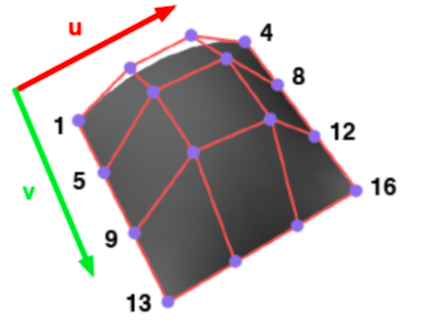
\includegraphics[width=.4\textwidth]{img/uv.png}
    \caption{\textit{Patch} de Bézier e respetivos pontos de controlo}
\end{figure}

Dependendo do nível de tesselação, serão calculados os vários pares $(u, v)$ que 
posteriormente serão escritos para um ficheiro \texttt{3d}, de modo a gerar triângulos que 
representam corretamente o modelo a desenhar. Assim, conclui-se que quanto maior o nível de 
tesselação, mais uniforme será o modelo gerado.

\

Deste modo, começou-se por definir as matrizes
necessárias:

\paragraph{Matrizes $a$ e $b$}

\begin{equation*}
    a = \begin{bmatrix}
        a^3 & a^2 & a & 1
        \end{bmatrix}
\end{equation*}

\begin{equation*}
    b = \begin{bmatrix}
        b^3 & b^2 & b & 1
        \end{bmatrix}
\end{equation*}

\paragraph{Matrizes com Pontos de Controlo}

\begin{equation*}
    P = \begin{bmatrix}
        P_{00} & P_{01} & P_{02} & P_{03} \\
        P_{10} & P_{11} & P_{12} & P_{13} \\
        P_{20} & P_{21} & P_{22} & P_{23} \\
        P_{30} & P_{31} & P_{32} & P_{33} 
        \end{bmatrix}
\end{equation*}

\paragraph{Matrizes de Bézier}

\begin{equation*}
    M = \begin{bmatrix}
        -1 & 3 & -3 & 1 \\
        3 & -6 & 3 & 0 \\
        -3 & 3 & 0 & 0 \\
        1 & 0 & 0 & 0
        \end{bmatrix}
\end{equation*}

\

Tendo por base os valores de $a$ e $b$, que se encontram contidos no intervalo $\left[ 0, 1 
\right]$, torna-se possível obter um ponto da superfície de Bézier, através da seguinte 
fórmula:

$$P(a, b) = a \times M \times P \times M \times b$$

Neste sentido, a função \texttt{getPoint}, que permite obter as coordenadas de um ponto, por 
aplicação desta expreesão. Para além disto, foi necessário elaborar a função 
\texttt{getPatchPoints} que, fazendo uso da função \texttt{getPoint}, é responsável por 
determinar as coordenadas dos vértices dos triângulos necessários à triangulação da figura.

\subsubsection*{Curvas de Bézier}

O processamento de \textit{patches} de Bézier é feito a partir do conceito de curvas de Bézier. 
Assim, a curva Bézier é definida em função de um parâmetro $t$, designado por Tesselação, 
que varia entre 0 e 1, ou seja para qualquer valor de $t$ no intervalo $\left[ 0, 1 \right]$, o 
valor da função nesse ponto representa um ponto da curva no espaço tridimensional. Para se 
calcular a curva completa, é necessário calcular os pontos da curva à medida que se incrementa o 
valor de $t$.

Para obter estas curvas, é necessário recorrer a quatro pontos de controlo -- $P_0$, $P_1$, $P_2$ 
e $P_3$. Estes, utilizados numa função juntamente com um parâmetro $t$, tornam possível a 
criação de uma curva. De seguida, poderá observar-se a fórmula que define uma curva de Bézier, 
bem como um exemplo de uma curva.

$$P(t) = (1 - t^3)P_0 + 3t(1 - t^2)P_1 + 3t^2(1 - t)P_2 + t^3P_3$$

\begin{figure}[H]
    \centering
    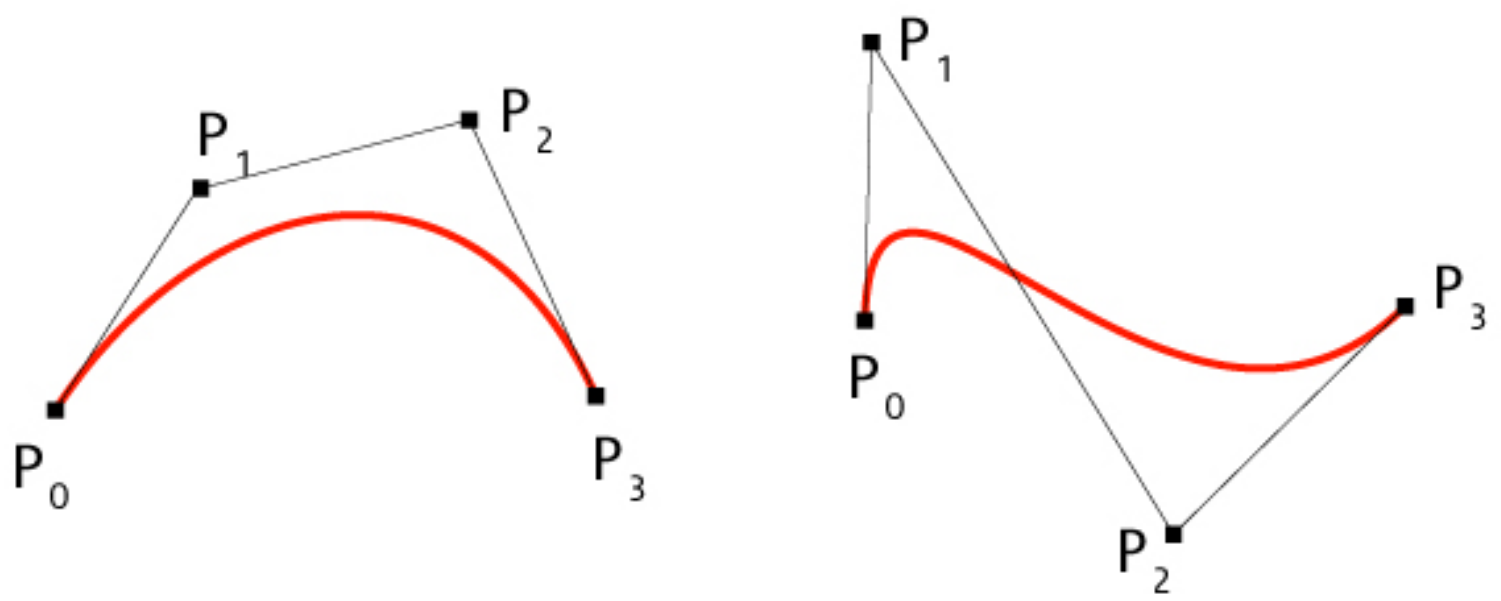
\includegraphics[width=.7\textwidth]{img/bezier_curve.png}
    \caption{Curvas de Bézier e respetivos pontos de controlo}
\end{figure}

Tendo em vista a obtenção de uma curva mais pormenorizada, deverá recorrer-se ao uso de um maior 
número de pontos, por forma a definir mais corretamente a curva.

\pagebreak

\section{\textit{Engine}}

O objetivo do \textit{engine} continua a ser o mesmo -- permitir a apresentação de uma janela e 
exibição dos modelos requisitados. Além disso, permite, também, a interação com os mesmos a 
partir de certos comandos. Tal como na fase anterior do trabalho prático, existe um ficheiro XML 
que vai ser interpretado. No entanto, para esta fase do projeto, a arquitetura deste ficheiro 
evolui de maneira a cumprir os requisitos. Desta forma, foram feitas algumas alterações nos 
métodos de \textit{parsing} e consequentemente alterações nas medidas de armazenamento e também 
de renderização.

\subsection{Alterações no ficheiro XML}

O ficheiro XML sofreu diversas mudanças, de forma ser capaz de respeitar os requisitos para esta 
fase do trabalho prático.

\subsubsection{Translação}
\label{sec:xml_trans}

Para definir uma translação animada, cria-se um bloco \textit{translate} com o parâmetro 
\texttt{time}, e dentro deste define se a lista de pontos que a translação ira seguir, tal como 
se pode ver de seguida..

\begin{minted}{xml}
<translate time="10">
   <point X="25.000000" Y="0.000000" Z="0.000000" />
   <point X="23.096989" Y="0.000000" Z="9.567086" />
   <point X="17.677670" Y="0.000000" Z="17.677670" />
</translate>
\end{minted}

\subsubsection{Rotação}
\label{sec:xml_rot}

Uma rotação animada troca apenas o ângulo por uma duração, que indica o tempo, em segundos, 
necessário para uma rotação de \SI{360}{\degree}, como se pode ver de seguida.

\begin{minted}{xml}
<rotate time="10" Y="1" />
\end{minted}

\subsection{VBOs}

Os VBOs oferecem um aumento na \textit{performance} em comparação com o modo de renderização 
imediata, devido ao facto de os dados serem armazenados na memória gráfica em vez de na memória 
do sistema, sendo diretamente renderizados pelo GPU. 

Extraída a informação relativa a uma figura, neste caso as coordenadas dos seus vértices, os 
quais provêm de um ficheiro \texttt{3d}, esta é utilizada para inicializar e preencher o 
\textit{buffer} relativo à figura em questão. Note-se que foi implementado um VBO por figura -- 
\textit{i.e.} por cada instância da classe \texttt{Shape}-- pois estas são independentes umas das 
outras, na sua maioria.

Logo após a leitura do ficheiro com os pontos, estes ficam guardados num vetor. Este último é 
percorrido, inserindo os vértices num \textit{array} que é utilizado no VBO da figura em questão.

\subsubsection{Classe \texttt{Shape}}

O OpenGL permite o uso de VBOs por forma a inserir toda a informação dos vértices diretamente na 
placa gráfica. Assim, começou-se por implementar os \textit{arrays} que contêm os vértices das 
primitivas a desenhar, bem como uma variável que indica o número de vértices que o 
\textit{buffer} contém.

\begin{minted}{cpp}
class Shape {
private:
    unsigned int nVertices;
    GLuint buffer[1];
    // (...)
};
\end{minted}

Aquando da instanciação de objetos desta classe, preenche-se o \textit{buffer} com os vértices 
que lhe são passados como argumento, guardando, também, na memória da placa gráfica 
\texttt{nVertices * 3} vértices.

\begin{minted}{cpp}
Shape::Shape(const vector<Vertex *> &vertices) {
    nVertices = vertices.size();
    float *vert = (float *)malloc(nVertices * 3 * sizeof(float));

    size_t i = 0;
    for (vector<Vertex *>::const_iterator v_it = vertices.begin();
         v_it != vertices.end(); ++v_it) {
        vert[i++] = (*v_it)->getX();
        vert[i++] = (*v_it)->getY();
        vert[i++] = (*v_it)->getZ();
    }

    glGenBuffers(1, buffer);
    glBindBuffer(GL_ARRAY_BUFFER, buffer[0]);
    glBufferData(GL_ARRAY_BUFFER, sizeof(float) * nVertices * 3, vert,
                 GL_STATIC_DRAW);

    free(vert);
}
\end{minted}

Por fim, por forma a desenhar a informação guardada, foi desenvolvdo o seguinte método, que 
desenha todos os vértices guardados, tornando possível aumentar o desempenho, sendo visível um 
aumento do número de \textit{frames} por segundo, em comparação aos obtidos quando os modelos 
são desenhados através de renderização imediata.

\begin{minted}{cpp}
void Shape::drawShape() {
    glBindBuffer(GL_ARRAY_BUFFER, buffer[0]);
    glVertexPointer(3, GL_FLOAT, 0, 0);
    glDrawArrays(GL_TRIANGLES, 0, nVertices);
}
\end{minted}

\subsection{Curvas de Catmull-Rom}

Um dos objetivos principais nesta fase consiste definir as órbitas dos planetas através da 
definição das curvas de Catmull-Rom.

\subsubsection{Classe \texttt{Transform}}

Relativamente à fase anterior do trabalho prático, foram adicionadas novas variáveis de 
instância à classe \texttt{Transform}, associadas a transformações novas que foram criadas. 
Para além disto, adicionaram-se funções e variáveis necessárias à implementação das curvas 
de Catmull-Rom.

\begin{minted}{cpp}
class Transform {
private:
    std::string type;
    float angle, x, y, z, time;
    std::vector<Vertex *> controlPoints, pointsCurve;
    bool deriv;
    float vector[4] = {1, 0, 0};
    // (...)
};
\end{minted}

De modo a representar as estas curvas, utilizou-se a \textit{spline} de Catmull-Rom. Para a 
definição da curva serão necessários pelo menos quatro pontos.

Assim, considerando que o valor de $t$ está contido no intervalo $\left[ 0, 1 \right]$, as 
coordenadas de um ponto da curva e a sua derivada são dadas por:

\begin{equation*}
    P(t) = \begin{bmatrix} t^3 & t^2 & t & 1 \end{bmatrix}
           \begin{bmatrix}
        -0.5 & 1.5 & -1.5 & 0.5 \\
        1 & -2.5 & 2 & -0.5 \\
        -0.5 & 0 & 0.5 & 0 \\
        0 & 1 & 0 & 0
        \end{bmatrix}
           \begin{bmatrix} P_0 \\ P_1 \\ P_2 \\ P_3 \end{bmatrix}
\end{equation*}

\

\begin{equation*}
    P'(t) = \begin{bmatrix} 3t^2 & 2t & 1 & 0 \end{bmatrix}
    \begin{bmatrix}
        -0.5 & 1.5 & -1.5 & 0.5 \\
        1 & -2.5 & 2 & -0.5 \\
        -0.5 & 0 & 0.5 & 0 \\
        0 & 1 & 0 & 0
        \end{bmatrix}
            \begin{bmatrix} P_0 \\ P_1 \\ P_2 \\ P_3 \end{bmatrix}
\end{equation*}

\

Desta forma, será possível obter um modelo do Sistema Solar dinâmico. Como tal, implementou-se a 
função \texttt{getGlobalCatmullRomPoint} que permitirá a obtenção de coordenadas dos pontos e 
as suas derivadas. Esta função recorre à função auxiliar \texttt{getCatmullRomPoint}, que 
utiliza as matrizes e vetores referidos anteriormente, por forma a gerar os valores de retorno.

Com o intuito de crir as órbitas dos planetas, defiu-se a função \texttt{setCatmullPoints}, os 
pontos da curva a partir dos pontos lidos no ficheiro XML, recorrendo à função 
\texttt{getGlobalCatmull}\ \texttt{RomPoint}, uma vez que esta permite obter as coordenadas do 
próximo ponto da curva para um dado valor $t$. Deste modo, percorre-se um ciclo que começa em 0 e 
termina em 1, usando incrementos de 0.01, por forma a gerar 100 pontos da curva.

\begin{minted}{cpp}
void Transform::setCatmullPoints() {
    float ponto[4];
    float der[4];

    for (float i = 0; i < 1; i += 0.01) {
        getGlobalCatmullRomPoint(i, ponto, der);
        Vertex *p = new Vertex(ponto[0], ponto[1], ponto[2]);
        pointsCurve.push_back(p);
    }
}
\end{minted}

Tendo as coordenadas dos pontos da curva, a função \texttt{drawOrbits} é responsável pelo 
desenho da curva

\begin{minted}{cpp}
void drawOrbits(Transform *t) {
    glColor3f(1.0f, 1.0f, 1.0f);
    glBegin(GL_LINE_LOOP);
    for (Vertex *p : t->getPointsCurve()) {
        glVertex3f(p->getX(), p->getY(), p->getZ());
    }
    glEnd();
}
\end{minted}

\subsection{Movimento dos Planetas}

Recorrendo ao uso de transformações geométricas, tais como rotações e translações, tornou-se 
possível dotar os planetas de movimento relativamente a outra figura ou a eles próprios. 


Assim, foram criada novas variáveis globais, por forma a capacitar o utilizador da capacidade de 
parar e retomar o movimento dos planetas, assim como alterar a velocidade do movimento.

Desta forma, são utilizados os diferentes tipos de rotações e translações descritos 
anteriormente. Esta movimentação tem por base o decorrer do tempo de vida da aplicação, sendo 
este o impulsionador do movimento de todas as figuras. Neste sentido, foram criadas as seguintes 
variáveis globais:

\begin{itemize}
    \item \texttt{eTime} --  Tempo decorrido desde que o movimento dos planetas está ativo;
    \item \texttt{cTime} -- Tempo decorrido desde que o programa foi iniciado.
    \item \texttt{speed} -- Variável utilizada para controlar a velocidade da animação:
    \item \texttt{stop} -- Variável que controla a existência ou ausência de movimentação. 
Tomará o valor \texttt{false} caso o movimento esteja ativo, ou o valor \texttt{true}, caso o 
movimento
    esteja inativo.
\end{itemize}

\pagebreak

\subsubsection{Transformações Geométricas}

Para aplicar as transformações geométricas, foi necessário definir a função 
\texttt{apply\_trans}, que, após a sua leitura dos ficheiros XML, irá aplicar estas 
transformações.

\subsubsection*{Rotação}

Por forma a implementar o movimento de rotação dos planetas, que lhes permite rodar sobre o 
próprio eixo, foi necessário adicionar a variável \texttt{time} à classe \texttt{Transform}, 
que indica o tempo que uma figura demora a realizar uma rotação completa sobre o seu próprio 
eixo. Por forma a utilizar esta variável eficazmente, foi necessário também alterar a função 
\texttt{parseRotate} de modo a acomodar estas alterações.

Novamente, é necessário recorrer à variável \texttt{eTime} de forma a determinar o tempo já 
decorrido durante a movimentação dos planetas. Recorrendo à multiplicação deste valor pelo 
valor do ângulo de rotação, obtêm-se diferentes ângulos à medida que o tempo passa. Assim, 
torna-se possível dotar a figura de um movimento de rotação sobre o seu próprio eixo. Tendo 
tudo isto em causa, definiu-se o seguinte excerto de código para o processamento das 
transformações de movimento de rotação.

\begin{minted}{cpp}
if (!strcmp(type, "rotateTime")) {
    float aux = eTime * angle;
    glRotatef(aux, x, y, z);
}
\end{minted}

\subsubsection*{Translação}

Foi também necessário capacitar os planetas de um movimento de translação em torno do Sol, 
usando para isso, também, a variável \texttt{time} referida anteriormente. Neste caso, esta 
variável define o tempo necessário para que uma determinada figura ou grupo percorra a curva 
definida pelos seus pontos de controlo, contidos no nodo \texttt{translate}. Para aplicar este 
movimento, foi necessário alterar a função \texttt{parseTranslate},
de modo a acomodar estas alterações.

Tal como mencionado na secção \ref{sec:xml_trans}, o tempo de translação é passado como 
parámetro no ficheiro XML. O objetivo consiste em que, com o decorrer do tempo, o planeta se 
desloque ao longo da sua órbita, aplicando o movimento de translação desejado. Para tal ser 
possível, recorremos à variável \texttt{eTime}, que guarda o tempo decorrido enquanto que o 
sistema se encontrava em movimento, e ainda à função \texttt{getGlobalCatmullRomPoint}.

Para além de tudo isto, a função \texttt{apply\_trans} terá também uma condição que será 
utilizada para definir a trajetória do cometa. Este deverá não só mover-se segundo a sua 
trajetória, como também manter se na orientação da curva. Deste modo, no caso do cometa e de 
outras figuras que se pretenda que o movimento seja descrito desta forma, o ficheiro XML deverá 
conter a informação disposta da seguinte forma:

\pagebreak

\begin{minted}{xml}
<translate time="250" derivative="1">
    <point X="250.000000" Y="0.000000" Z="0.000000" />
    <point X="0.000000" Y="0.000000" Z="250.000000" />
    <point X="-250.000000" Y="0.000000" Z="0.000000" />
    <point X="-100.000000" Y="0.000000" Z="-100.000000" />
    <point X="0.000000" Y="0.000000" Z="-250.000000" />
</translate>
\end{minted}

Surge agora aparece um parâmetro novo -- a derivada do ponto da curva. De forma a que o cometa 
esteja orientado, é necessário criar uma matriz que irá ser utilizada na função 
\texttt{glMultMatrixf}, com o objetivo de manter o cometa alinhado com a curva.

Desta forma, o seguinte excerto é responsável pelos movimentos de translação.

\begin{minted}{cpp}
if (!strcmp(type, "translateTime")) {
    float p[4], d[4];
    float dTime = eTime * time;

    t->getGlobalCatmullRomPoint(dTime, p, d);

    drawOrbits(t);
    glTranslatef(p[0], p[1], p[2]);

    if (t->isDeriv()) {
        float res[4];
        t->normalize(d);
        t->cross_product(d, t->getVector(), res);
        t->normalize(res);
        t->cross_product(res, d, t->getVector());
        float matrix[16];
        t->normalize(t->getVector());
        t->rotMatrix(matrix, d, t->getVector(), res);
        glMultMatrixf(matrix);
    }
}
\end{minted}

Note-se que na aplicação das transformações geométricas foi utilizada a função 
\texttt{glutGet(GLUT\_}\\\texttt{ELAPSED\_TIME)} para o cálculo do tempo passado para que desta 
forma a velocidade dos planetas não esteja dependente da \textit{frame rate} do programa.

\pagebreak

\section{Análise de Resultados}

\subsection{\textit{Teapot}}

De seguida, apresentam-se imagens que representam a renderização um \textit{teapot} com valores 
de tesselação de 2 e 10, respetivamente, criados a partir do ficheiro \texttt{teapot.patch} 
fornecido, e utilizando as novas funcionalidades do \textit{generator}, que permitem criar pontos 
através de \textit{patches} de Bézier.

\begin{figure}[H]
\centering
\begin{subfigure}{.5\textwidth}
    \centering
    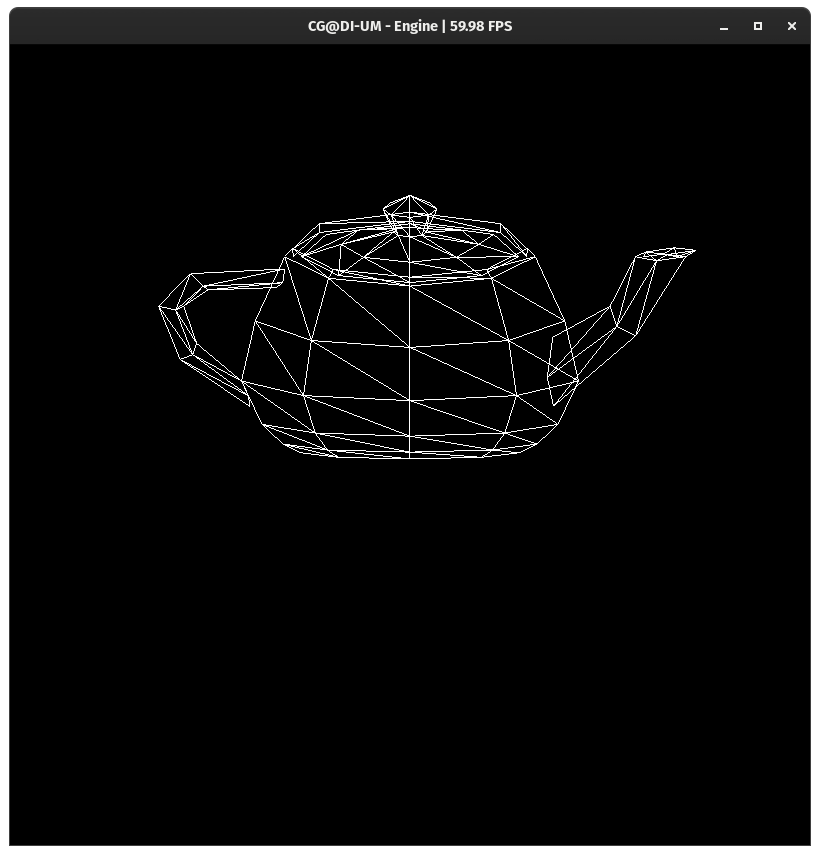
\includegraphics[width=\textwidth]{img/teapot2.png}
    \caption{\textit{Teapot} renderizado com um nível de \\ tesselação igual a 2}
\end{subfigure}%
\begin{subfigure}{.5\textwidth}
    \centering
    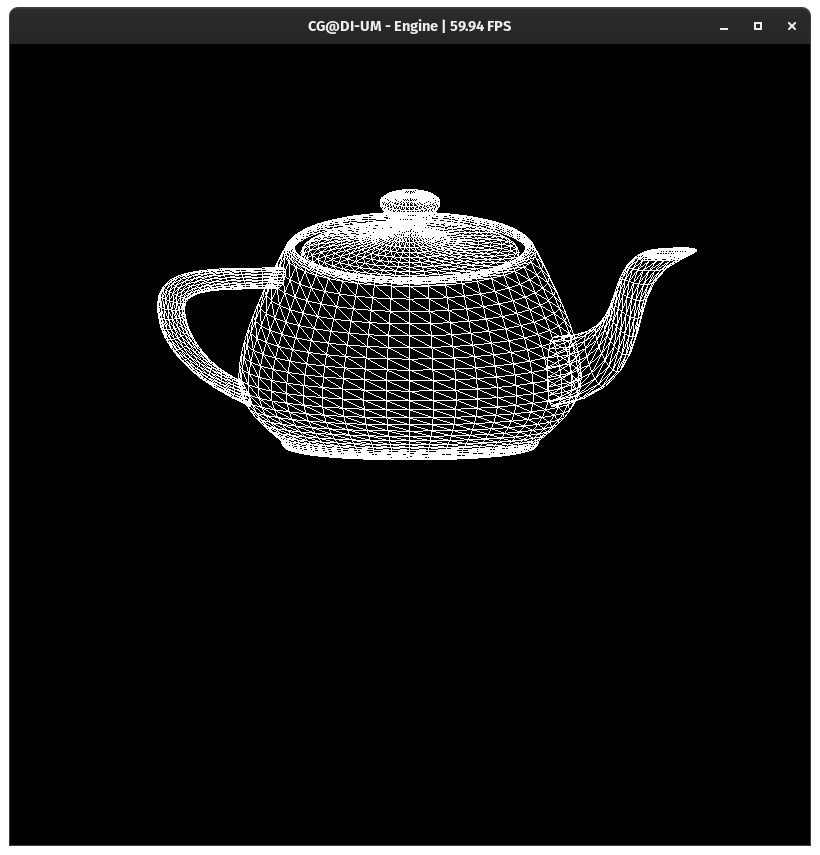
\includegraphics[width=\textwidth]{img/teapot10.png}
    \caption{\textit{Teapot} renderizado com um nível de \\ tesselação igual a 10}
\end{subfigure}
\caption{Renderização de um \textit{teapot} a partir de \textit{patches} de Bézier}
\end{figure}

\subsection{Modelo do Sistema Solar}

No modelo do Sistema Solar, cada um dos astros tem a sua própria órbita e esta é animada, à 
excepção do Sol.

De facto, todos os planetas foram representados com o máximo de cuidado no sentido de respeitar 
diferenças de tamanho e distância, mas sem nunca perder de vista que se trata de uma animação e 
que, por isso, não consegue nem deve respeitar a 100\% a escala real. Os movimentos de rotação e 
translação foram representados tentando também uma aproximação o mais possível à realidade. 
Houve ainda a preocupação de adicionar um cometa gerado através de um ficheiro de \textit{input} 
de um \textit{patch} de Bézeier para demonstrar também as capacidades do \textit{generator}.

\begin{figure}[H]
    \centering
    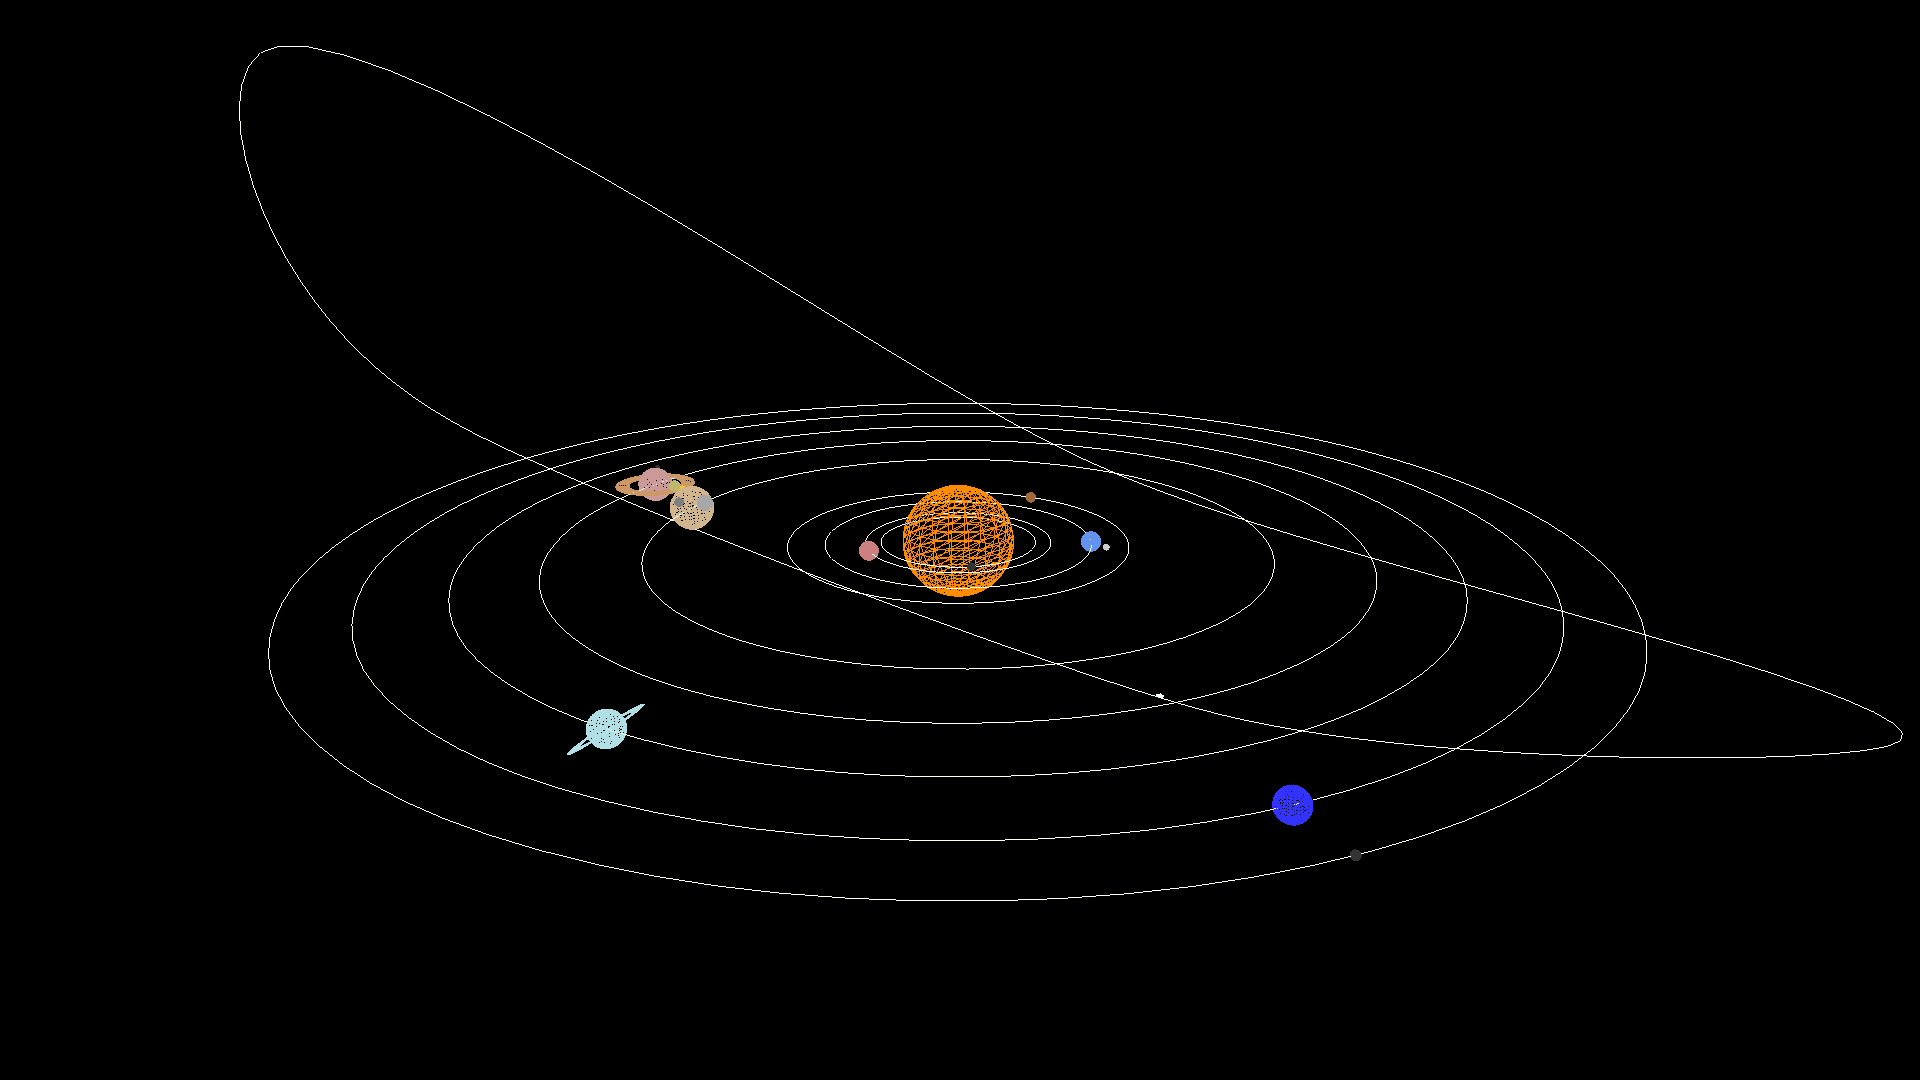
\includegraphics[width=\textwidth]{img/lines.png}
    \caption{Modelo do Sistema Solar renderizado com linhas}
\end{figure}

\vspace{1cm}

\begin{figure}[H]
    \centering
    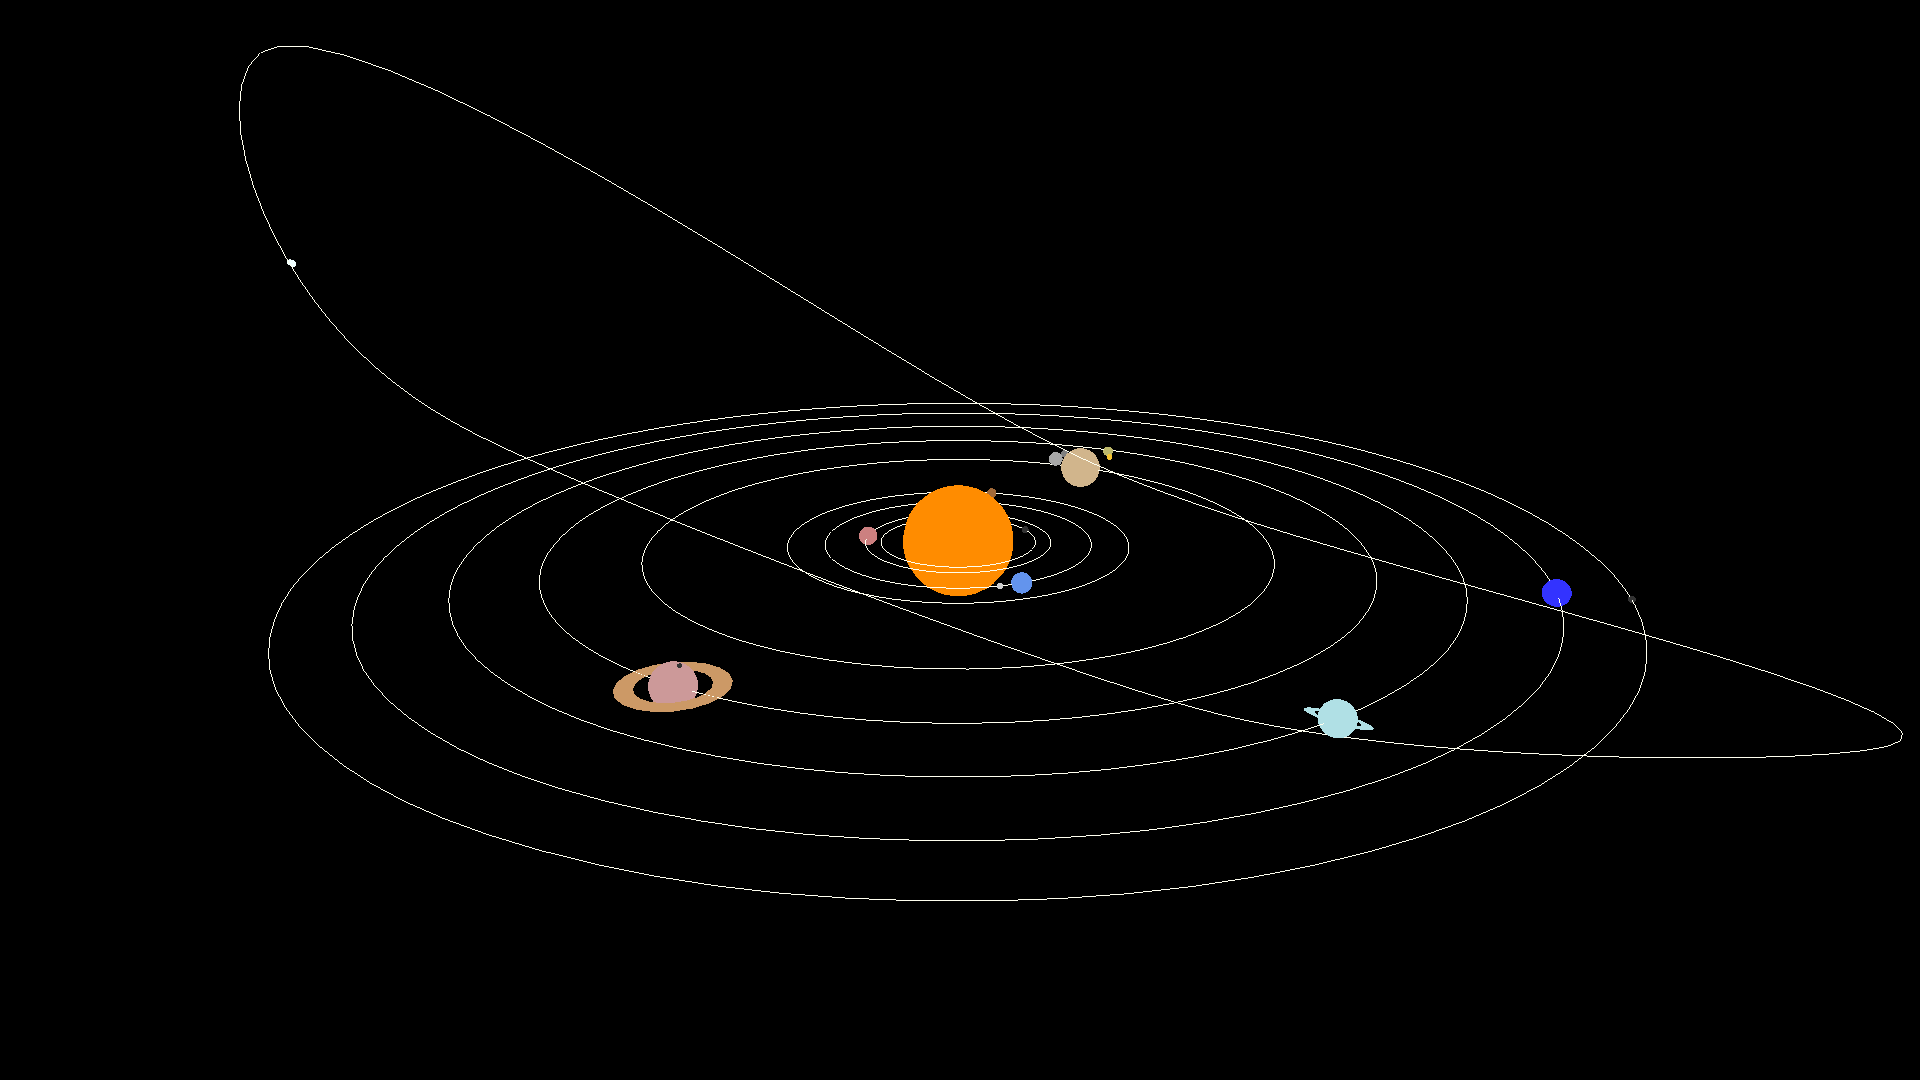
\includegraphics[width=\textwidth]{img/filled.png}
    \caption{Modelo do Sistema Solar renderizado com as figuras preenchidas}
\end{figure}

\begin{figure}[H]
    \centering
    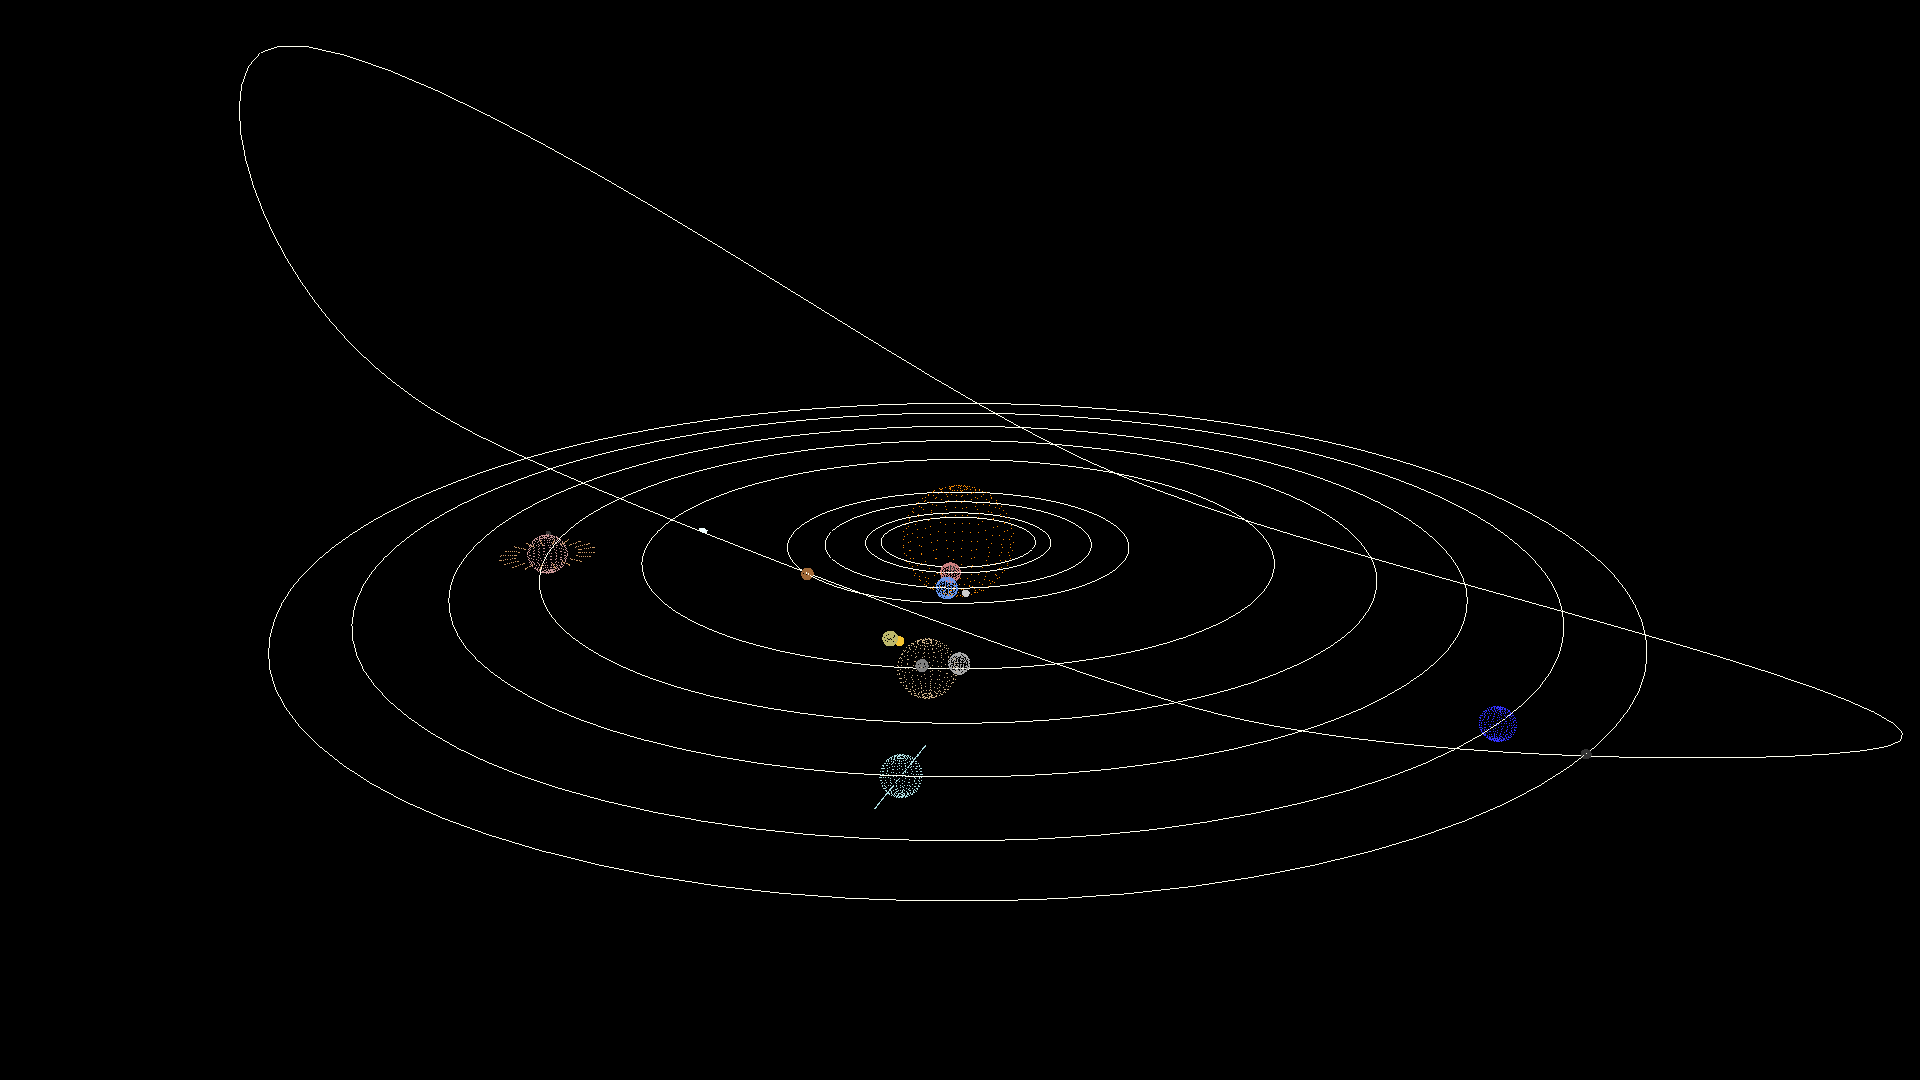
\includegraphics[width=\textwidth]{img/points.png}
    \caption{Modelo do Sistema Solar renderizado com pontos}
\end{figure}

\pagebreak

\subsection{\textit{Performance}}

Tal como referido anteriormente, o uso de VBOs permite aumentar de forma significativa o desempenho 
do programa, sendo visível um aumento do número de \textit{frames} por segundo em comparação 
aos verificados quando se renderiza a mesma \textit{scene} mas, desta vez, em que os modelos eram 
desenhados de uma forma mais primitiva -- através de renderização imediata -- tal como se pode 
ver de seguida.

Importa salientar que esta medição de \textit{performance} foi realizada tendo o \textit{vertical 
sync} desligado, de forma a garantir que os resultados obtidos não estejam limitados pela 
sincronização vertical.

\

\

\begin{figure}[H]
    \centering
    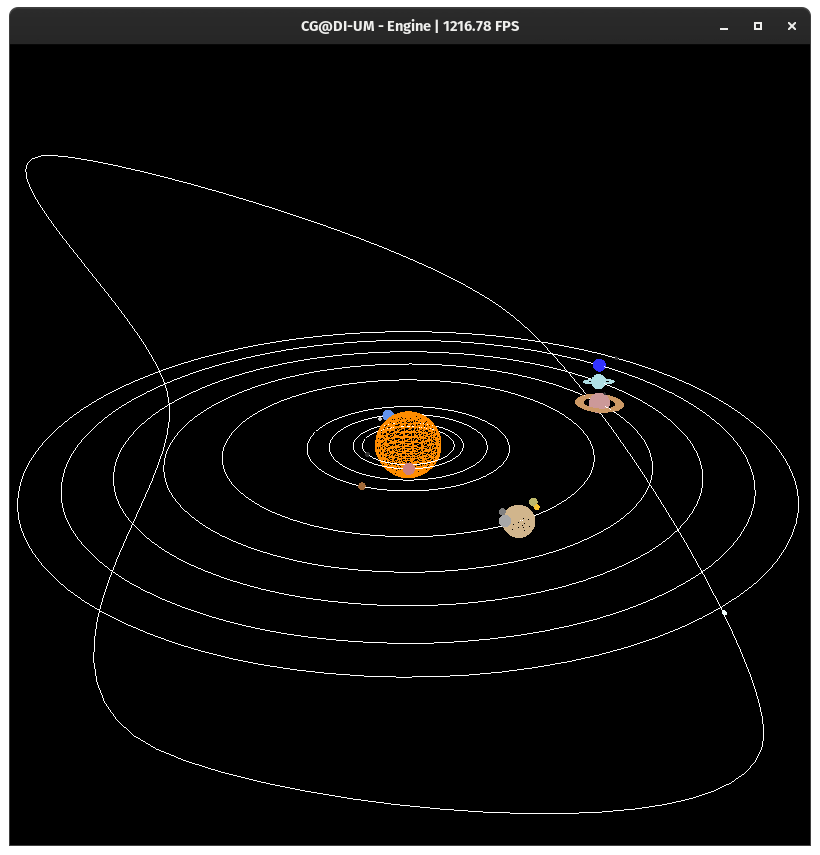
\includegraphics[width=.6\textwidth]{img/fps_comvbo.png}
    \caption{Modelo dinâmico do Sistema Solar renderizado \\ com \textit{Vertex Buffer Objects}}
\end{figure}

\begin{figure}[H]
    \centering
    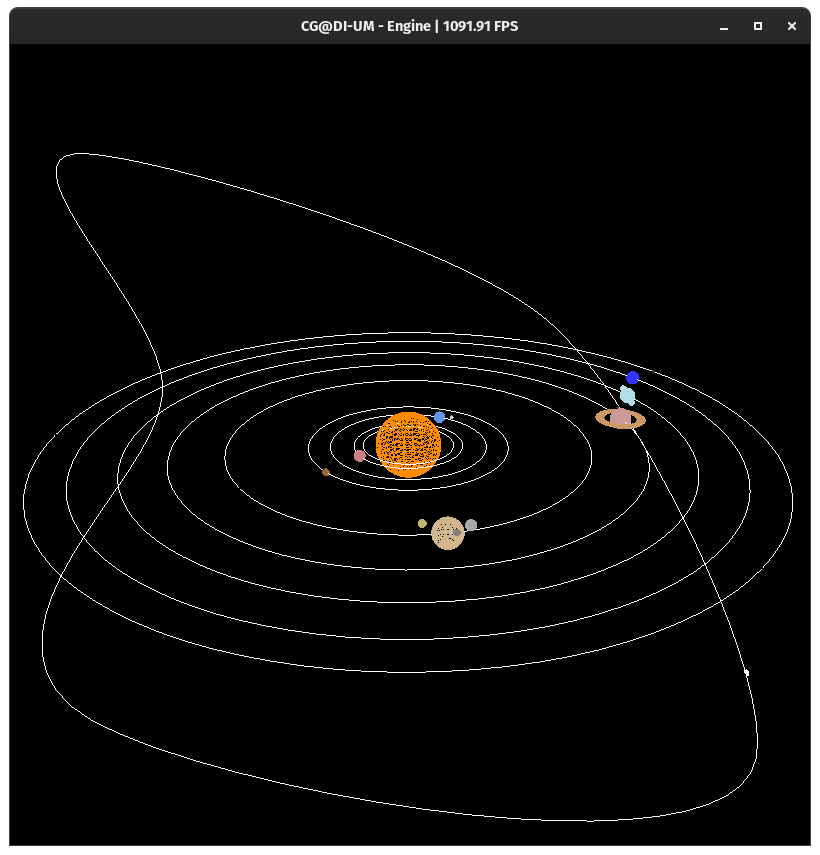
\includegraphics[width=.6\textwidth]{img/fps_semvbo.png}
    \caption{Modelo dinâmico do Sistema Solar renderizado \\
    através de renderização imediata}
\end{figure}

\pagebreak

\section{Conclusão}

Esta terceira fase do trabalho prático permitiu assimilar conhecimento relativamente aos processos 
de representação de figuras em Computação Gráfica. Este conhecimento foi adquirido através da 
matemática envolvente por detrás da renderização de imagens e o modo como o OpenGL processa a 
informação. Permitiu-nos descobrir como gerar objetos, ou efetuar transformações sobre eles 
através de pontos de controlo e outros dados relativos. Neste caso, através de \textit{patches} 
de Bézier e de curvas Catmull-Rom.

Para além disso, permitiu implementar um novo modo de gerar objetos, recorrendo a \textit{buffers} 
e adquirir conhecimento com estes.

Com a elaboração desta fase do projeto prático foi possível aplicar conhecimentos teóricos e 
práticos relativos tanto às curvas de Bézier como às de Catmull-Rom utilizadas para efetuar 
transformações sobre os objetos através de pontos de controlo e outros dados relativos, assim 
como o uso de VBOs para o desenho das primitivas gráficas.

Assim, considerámos que o resultado final desta fase corresponde às expectativas, na medida em 
que conseguimos desenvolver um modelo, agora dinâmico, do Sistema
Solar, tal como era pedido no enunciado. De facto, todas as funcionalidades pedidas foram 
implementadas. No entanto, algumas optimizações não foram implementadas, como por exemplo, o uso 
de índices nos VBOs. 

Desta forma, esperamos que para a próxima e última fase que se avizinha, consigamos concluir o 
projeto de forma a obter um resultado final ainda mais realista e visualmente agradável ao 
utilizador.

\pagebreak

\bibliographystyle{unsrt}
\bibliography{refs}

\end{document}
